\documentclass[t]{beamer}
%\documentclass[aspectratio=169]{beamer} % Соотношение сторон

%\usetheme{HSE}
%\usetheme{Berkeley} % Тема оформления
%%%% Работа с русским языком
%\usepackage{cmap}					% поиск в PDF
%\usepackage{mathtext} 				% русские буквы в формулах
%\usepackage[T2A]{fontenc}			% кодировка
%\usepackage[utf8]{inputenc}			% кодировка исходного текста
%\usepackage[english,russian]{babel}	% локализация и переносы

%% Beamer по-русски
\newtheorem{rtheorem}{Теорема}
\newtheorem{rproof}{Доказательство}
\newtheorem{rexample}{Пример}

%%% For commenting
\usepackage{verbatim}

%%% Дополнительная работа с математикой
\usepackage{amsmath,amsfonts,amssymb,amsthm,mathtools} % AMS
\usepackage{icomma}
%%% Работа с картинками
\usepackage{graphicx}  % Для вставки рисунков
%\graphicspath{{images/}{images2/}}  % папки с картинками
\setlength\fboxsep{3pt} % Отступ рамки \fbox{} от рисунка
\setlength\fboxrule{1pt} % Толщина линий рамки \fbox{}
\usepackage{wrapfig} % Обтекание рисунков текстом

%%% Работа с таблицами
\usepackage{array,tabularx,tabulary,booktabs} % Дополнительная работа с таблицами
\usepackage{longtable}  % Длинные таблицы
\usepackage{multirow} % Слияние строк в таблице

%%% Программирование
\usepackage{etoolbox} % логические операторы

%%% Другие пакеты
\usepackage{lastpage} % Узнать, сколько всего страниц в документе.
\usepackage{soul} % Модификаторы начертания
\usepackage{csquotes} % Еще инструменты для ссылок
%\usepackage[style=authoryear,maxcitenames=2,backend=biber,sorting=nty]{biblatex}
\usepackage{multicol} % Несколько колонок

%%% Картинки
\usepackage{tikz} % Работа с графикой
\usepackage{pgfplots}
\usepackage{pgfplotstable}


\graphicspath{{images/}}



%%% FOR TITLE BREAKS
\setbeamertemplate{frametitle continuation}{}


%%% FOR ALGORITHM
\usepackage{algorithm}
\usepackage{algpseudocode}
\usepackage{caption}

%\@addtoreset{algorithm}{chapter}% algorithm counter resets every chapter

% Перевод данных об алгоритмах

\renewcommand{\listalgorithmname}{Список алгоритмов}
\floatname{algorithm}{Алгоритм}

% Перевод команд псевдокода

\algrenewcommand\algorithmicwhile{\textbf{пока}}
\algrenewcommand\algorithmicdo{\textbf{выполнять}}
\algrenewcommand\algorithmicrepeat{\textbf{повторять}}
\algrenewcommand\algorithmicuntil{\textbf{пока выполняется}}
\algrenewcommand\algorithmicend{\textbf{Конец}}
\algrenewcommand\algorithmicif{\textbf{Если}}
\algrenewcommand\algorithmicelse{\textbf{иначе}}
\algrenewcommand\algorithmicthen{\textbf{тогда}}
\algrenewcommand\algorithmicfor{\textbf{Цикл}}
\algrenewcommand\algorithmicforall{\textbf{Выполнить для всех}}
\algrenewcommand\algorithmicfunction{\textbf{Функция}}
\algrenewcommand\algorithmicprocedure{\textbf{Процедура}}
\algrenewcommand\algorithmicloop{\textbf{Зациклить}}
\algrenewcommand\algorithmicrequire{\textbf{Вход:}}
\algrenewcommand\algorithmicensure{\textbf{Выход:}}
\algrenewcommand\algorithmicreturn{\textbf{Возвратить}}
\algrenewtext{EndWhile}{\textbf{конец цикла}}
\algrenewtext{EndLoop}{\textbf{Конец зацикливания}}
\algrenewtext{EndFor}{\textbf{Конец цикла}}
\algrenewtext{EndFunction}{\textbf{Конец функции}}
\algrenewtext{EndProcedure}{\textbf{Конец процедуры}}
\algrenewtext{EndIf}{\textbf{Конец условия}}
\algrenewtext{EndFor}{\textbf{Конец цикла}}
\algrenewtext{BeginAlgorithm}{\textbf{Начало алгоритма}}
\algrenewtext{EndAlgorithm}{\textbf{Конец алгоритма}}
\algrenewtext{BeginBlock}{\textbf{Начало блока. }}
\algrenewtext{EndBlock}{\textbf{Конец блока}}
\algrenewtext{ElsIf}{\textbf{иначе если }}


%%%FOR BIBLIOGRAPHY

\usepackage[backend=biber,bibencoding=utf8,sorting=nyt,maxcitenames=2,style=gost-numeric]{biblatex}

\addbibresource{reference.bib}

%%%%%%%%%%%%%%%%%%%%

\usefonttheme{default} % Font theme

\definecolor{HSEblue}{cmyk}{1,0.66,0,0.02}        % Pantone 286
\definecolor{HSEgreen}{cmyk}{0.69,0,1,0}          % Pantone 361
\definecolor{HSEred}{cmyk}{0,0.95,1,0.29}         % Pantone 484
\definecolor{HSEorange}{cmyk}{0,0.42,0.77,0}      % Pantone 131
\setbeamercolor{WhiteOnBlue}{bg=HSEblue,fg=white} % White on Pantone 286
\setbeamercolor{BlueOnWhite}{fg=HSEblue,bg=white} % Pantone 286 on White

%%% Some design features
\setbeamertemplate{navigation symbols}{}    % Comment out to show nav. bar
\setbeamertemplate{itemize items}[circle]

\usecolortheme[named=HSEblue]{structure}
\setbeamercolor{background canvas}{bg=white}
\setbeamercolor{frametitle}{bg=HSEblue}
\setbeamercolor{frametitle}{fg=white}
\setbeamercolor{headline}{bg=HSEblue}
\setbeamercolor{alerted text}{fg=HSEred}
\setbeamercolor{itemize item}{fg=HSEblue}
\setbeamercolor{itemize subitem}{fg=HSEblue}
\setbeamercolor{itemize subsubitem}{fg=HSEblue}
\setbeamercolor{block title example}{fg=HSEgreen}
\AtBeginEnvironment{exampleblock}{
	\setbeamercolor{itemize item}{fg=HSEgreen}
	\setbeamercolor{itemize subitem}{fg=HSEgreen}
	\setbeamercolor{itemize subsubitem}{fg=HSEgreen}
}
\setbeamercolor{palette primary}{bg=HSEblue}
\setbeamercolor{palette primary}{fg=white}
\setbeamercolor{palette secondary}{bg=HSEblue}
\setbeamercolor{palette secondary}{fg=white}
\setbeamercolor{palette tertiary}{bg=HSEblue}
\setbeamercolor{palette tertiary}{fg=white}

%%% Layout issues
%\setbeamertemplate{headline}[default]{} % Empty headline
\setbeamertemplate{frametitle} % Frametitle with logo
{
	\nointerlineskip
	\begin{beamercolorbox}[sep=0.3cm,wd=\paperwidth]{frametitle}
		\vbox{}\vskip-0.7ex%
		% \begin{wrapfigure}{r}{0.12\textwidth}
		% 	\vskip-3ex\includegraphics[width=0.08\textwidth]{HSE-theme/HSE-small}
		% \end{wrapfigure}
		\strut\insertframetitle

		\small\strut\insertframesubtitle
		\vskip-1ex%
	\end{beamercolorbox}
}

\makeatletter
\setbeamertemplate{footline} % Footline
{
	\leavevmode%
	\hbox{%
		\begin{beamercolorbox}[wd=.333333\paperwidth,ht=2ex,dp=1ex,center]{WhiteOnBlue}%
			\usebeamerfont{author in head/foot}\insertshortauthor
		\end{beamercolorbox}%
		\begin{beamercolorbox}[wd=.333333\paperwidth,ht=2ex,dp=1ex,center]{WhiteOnBlue}%
			\usebeamerfont{title in head/foot}\insertshortinstitute
		\end{beamercolorbox}%
		\begin{beamercolorbox}[wd=.333333\paperwidth,ht=2ex,dp=1ex,right]{WhiteOnBlue}%
			\usebeamerfont{date in head/foot}\insertshortdate{}\hspace*{2em}
			\insertframenumber{} / \inserttotalframenumber\hspace*{2ex}
		\end{beamercolorbox}}%
		\vskip0pt%
	}
	\makeatother

	\addtobeamertemplate{title page}{%
		\leavevmode%
		\vspace{-.23cm}
		\hbox{%
			\begin{beamercolorbox}[wd=\paperwidth,ht=0.2\paperheight]{frametitle}
				% \begin{center}
				% 	\includegraphics[height=0.28\paperheight]{HSE-theme/HSE-main}
				% 	\vspace{-0.025\paperheight}
				% \end{center}
			\end{beamercolorbox}}
		}{\vspace{3cm}}

%%%%%%%%%%%%%%%%%%%%%%%%%%%%

%\author{Аланов Айбек Арстанбекович}

\title[RL] % (optional, only for long titles)
{\textbf{Collision Avoidance Using Deep Reinforcement Learning}}
\author[]
{
	\footnotesize {\textbf{Team members}: Alexander Nekrashevich, Aibek Alanov, Dmitiy Salnikov}
}
\institute{}
\date{}

%\AtBeginSubsection[]
%{
%	\begin{frame}<beamer>{Contents}
%		\tableofcontents[currentsection,currentsubsection]
%	\end{frame}
%}


\begin{document}
{

\frame[plain]
{
	\titlepage
}
}

\section{Problem Formulation}

\begin{frame}
	\frametitle{\insertsection}
	Goals:
	\begin{itemize}
		\item Implement deep reinforcement learning algorithm
		\item Apply the algorithm for the collision avoidance problem
		\item Use AirSim framework and Unreal environment for the training
		\item Adapt the algorithm to each training environment
		\item Develop rewards and action spaces for each environment
	\end{itemize}
\end{frame}

\section{Deep Q-learning}

\begin{frame}
	\frametitle{\insertsection}
	\begin{itemize}
		\item We introduce the Q-function $Q: S \times A \to \mathbb{R}$.
		\item Learn it using the following loss:
		\begin{align*}
			L(\theta_i) = \mathbb{E}_{s,a,r,s'} \left[ \left(r + \gamma \max_{a'}Q(s', a'; \theta^{-}) - Q(s, a; \theta_i) \right)^2 \right]
		\end{align*}
		\item Our implementation uses deep learning libraries CNTK
and TensorFlow (with Tensorboard).
	\end{itemize}
\end{frame}

\begin{frame}
	\frametitle{Network Architecture}
	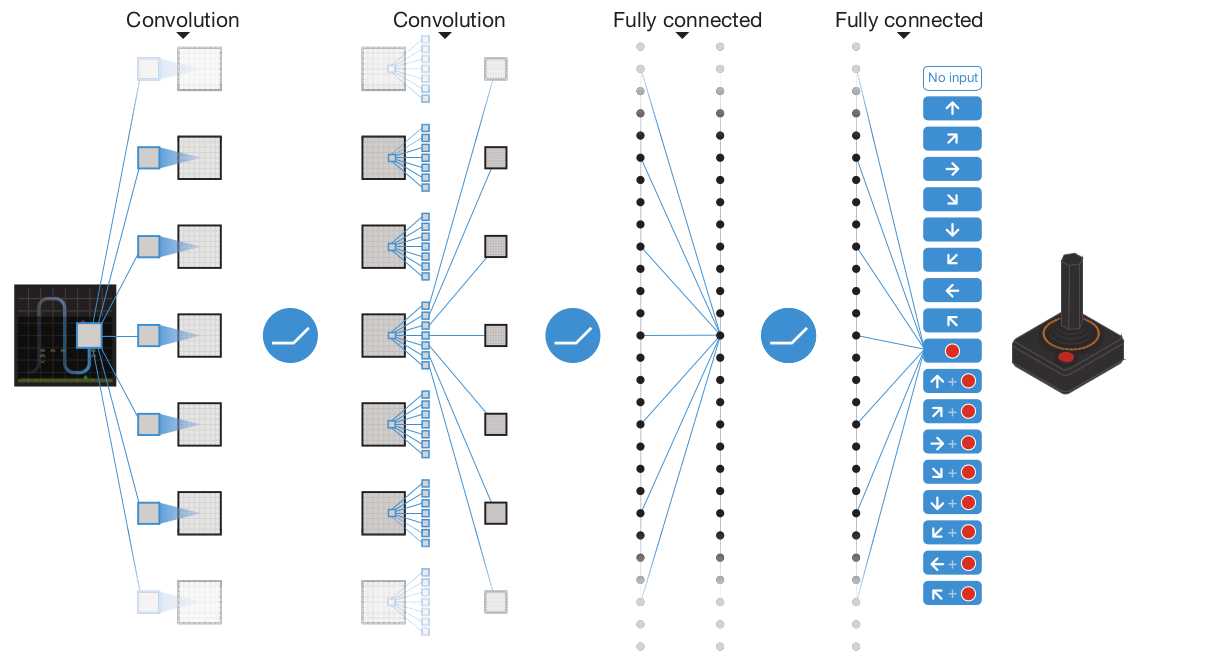
\includegraphics[scale=0.27]{images/dqn_crop.png}
\end{frame}

\section{Considered Environments}

\begin{frame}
	\frametitle{\insertsection}
	\begin{itemize}
		\item Blocks, Cave, Landscape Mountains, Corridor, City, Africa, Jing-Zha, Neighborhood.
	\end{itemize}
	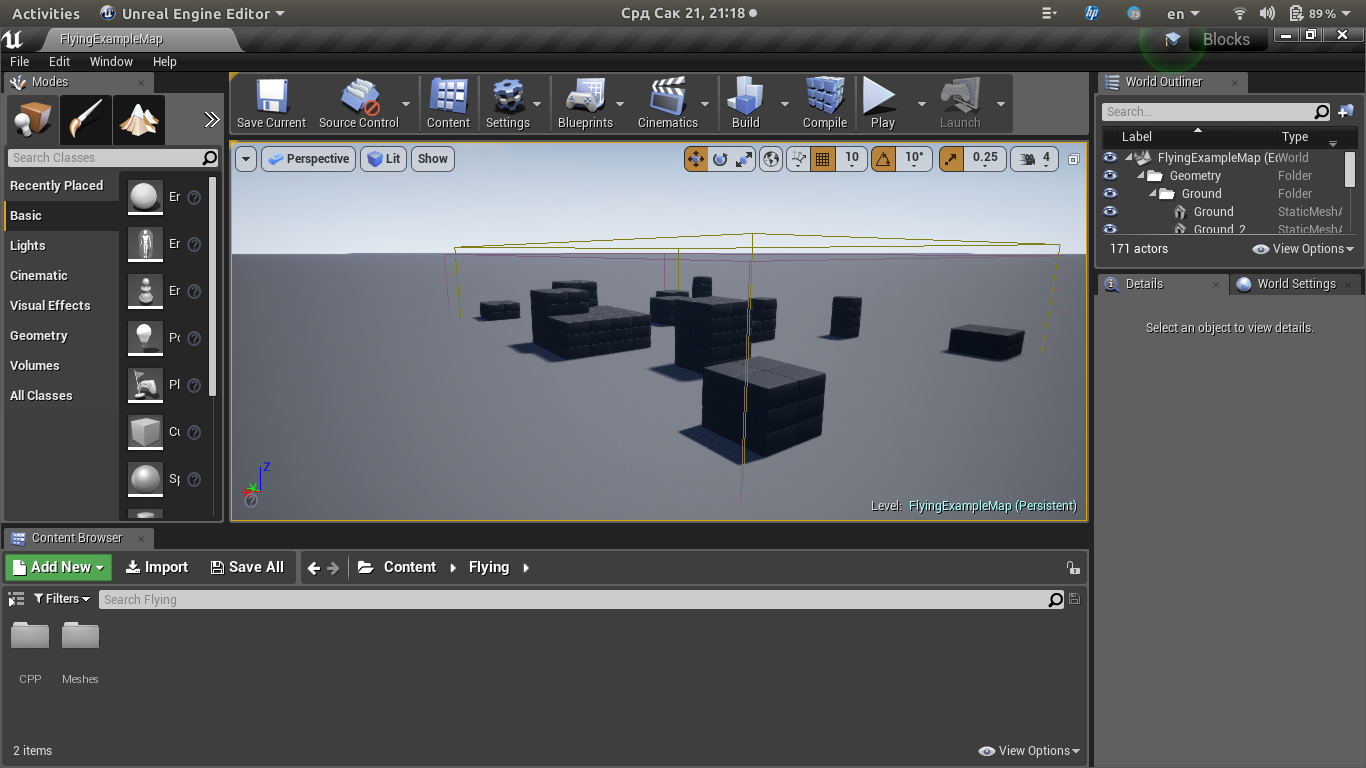
\includegraphics[scale=0.1]{images/blocks.png} $\quad$
	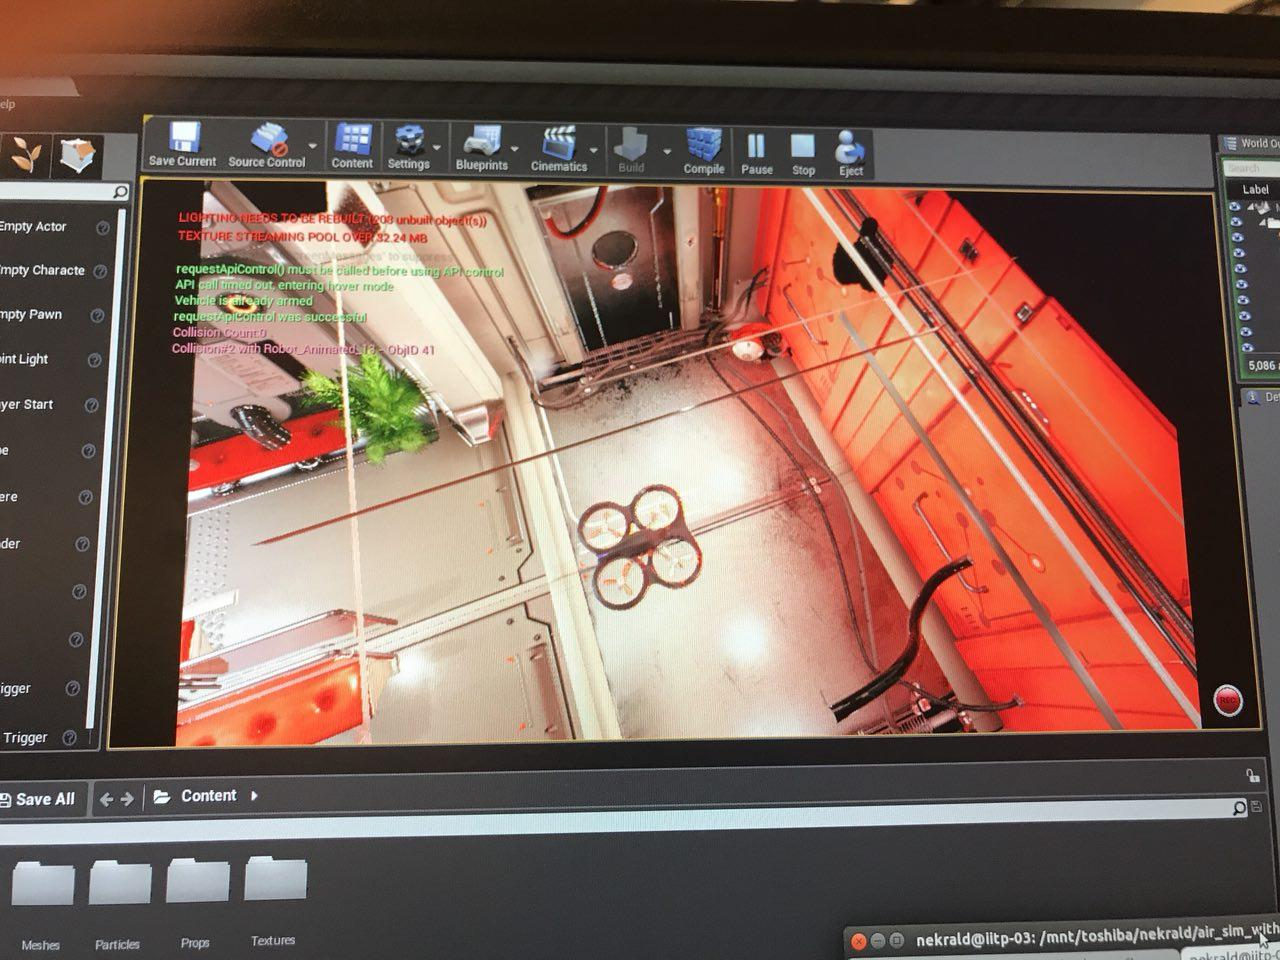
\includegraphics[scale=0.1]{images/corridor.jpg}

	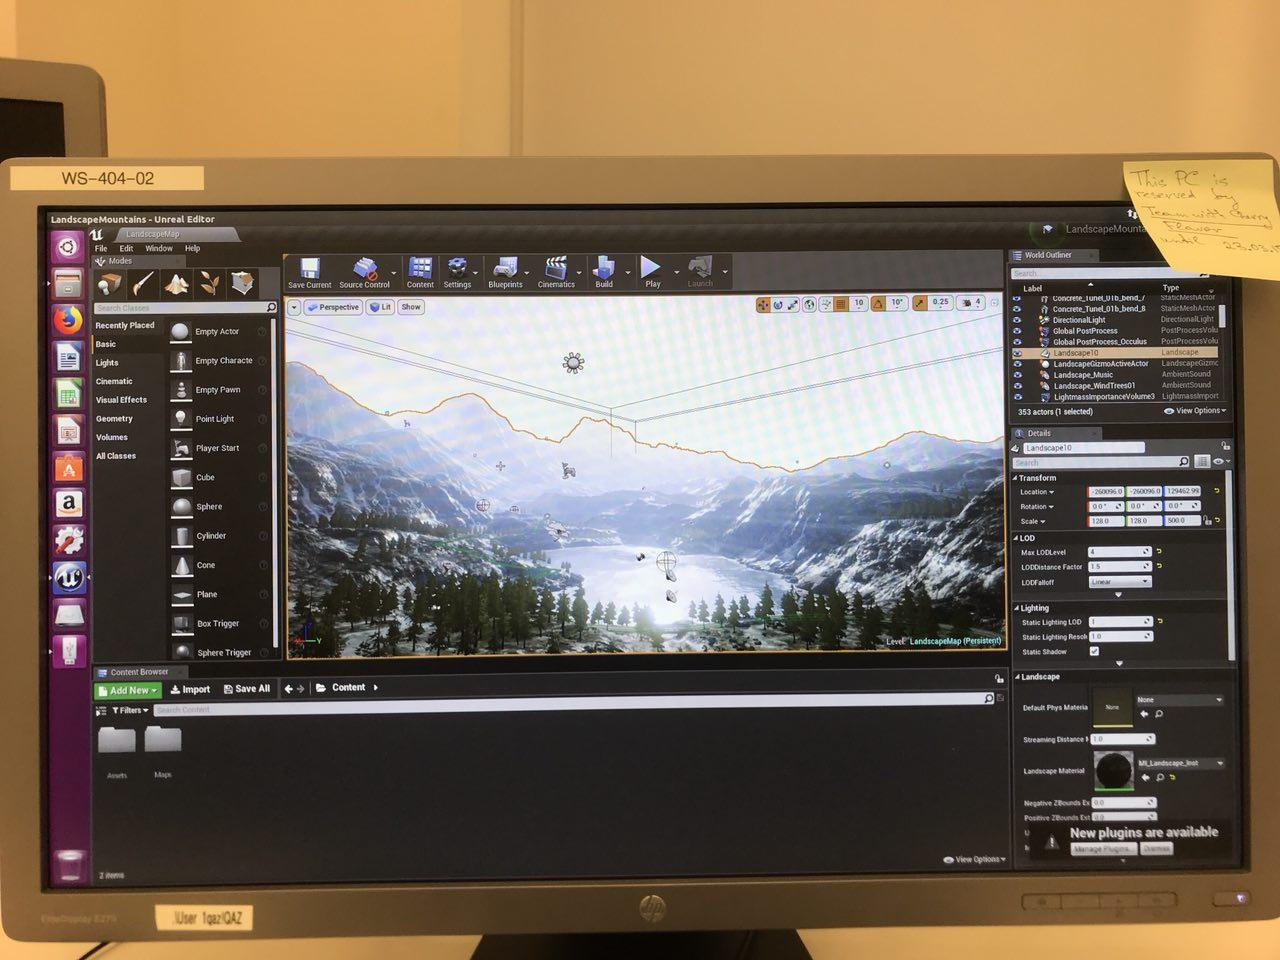
\includegraphics[scale=0.1]{images/landscape.jpg} $\quad$
	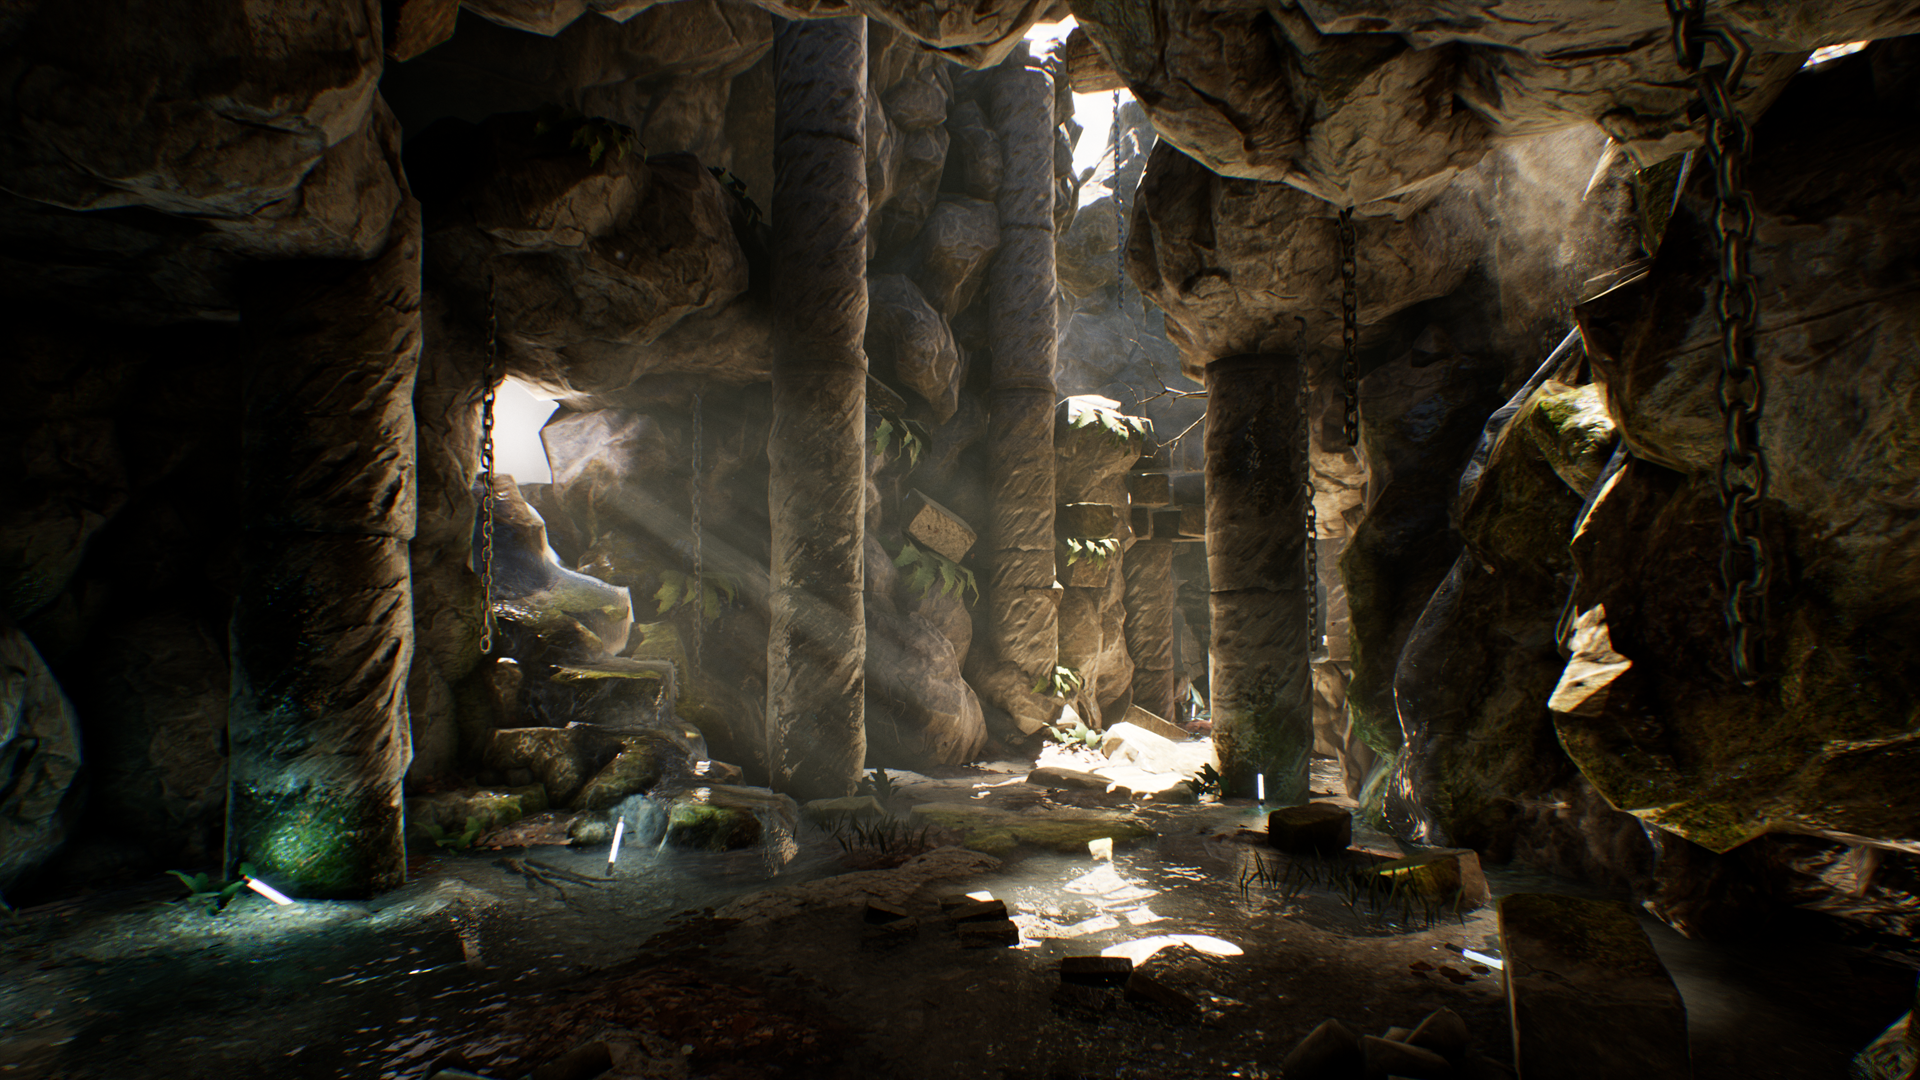
\includegraphics[scale=0.1]{images/cave.png}
\end{frame}

\begin{frame}
	\frametitle{\insertsection}
	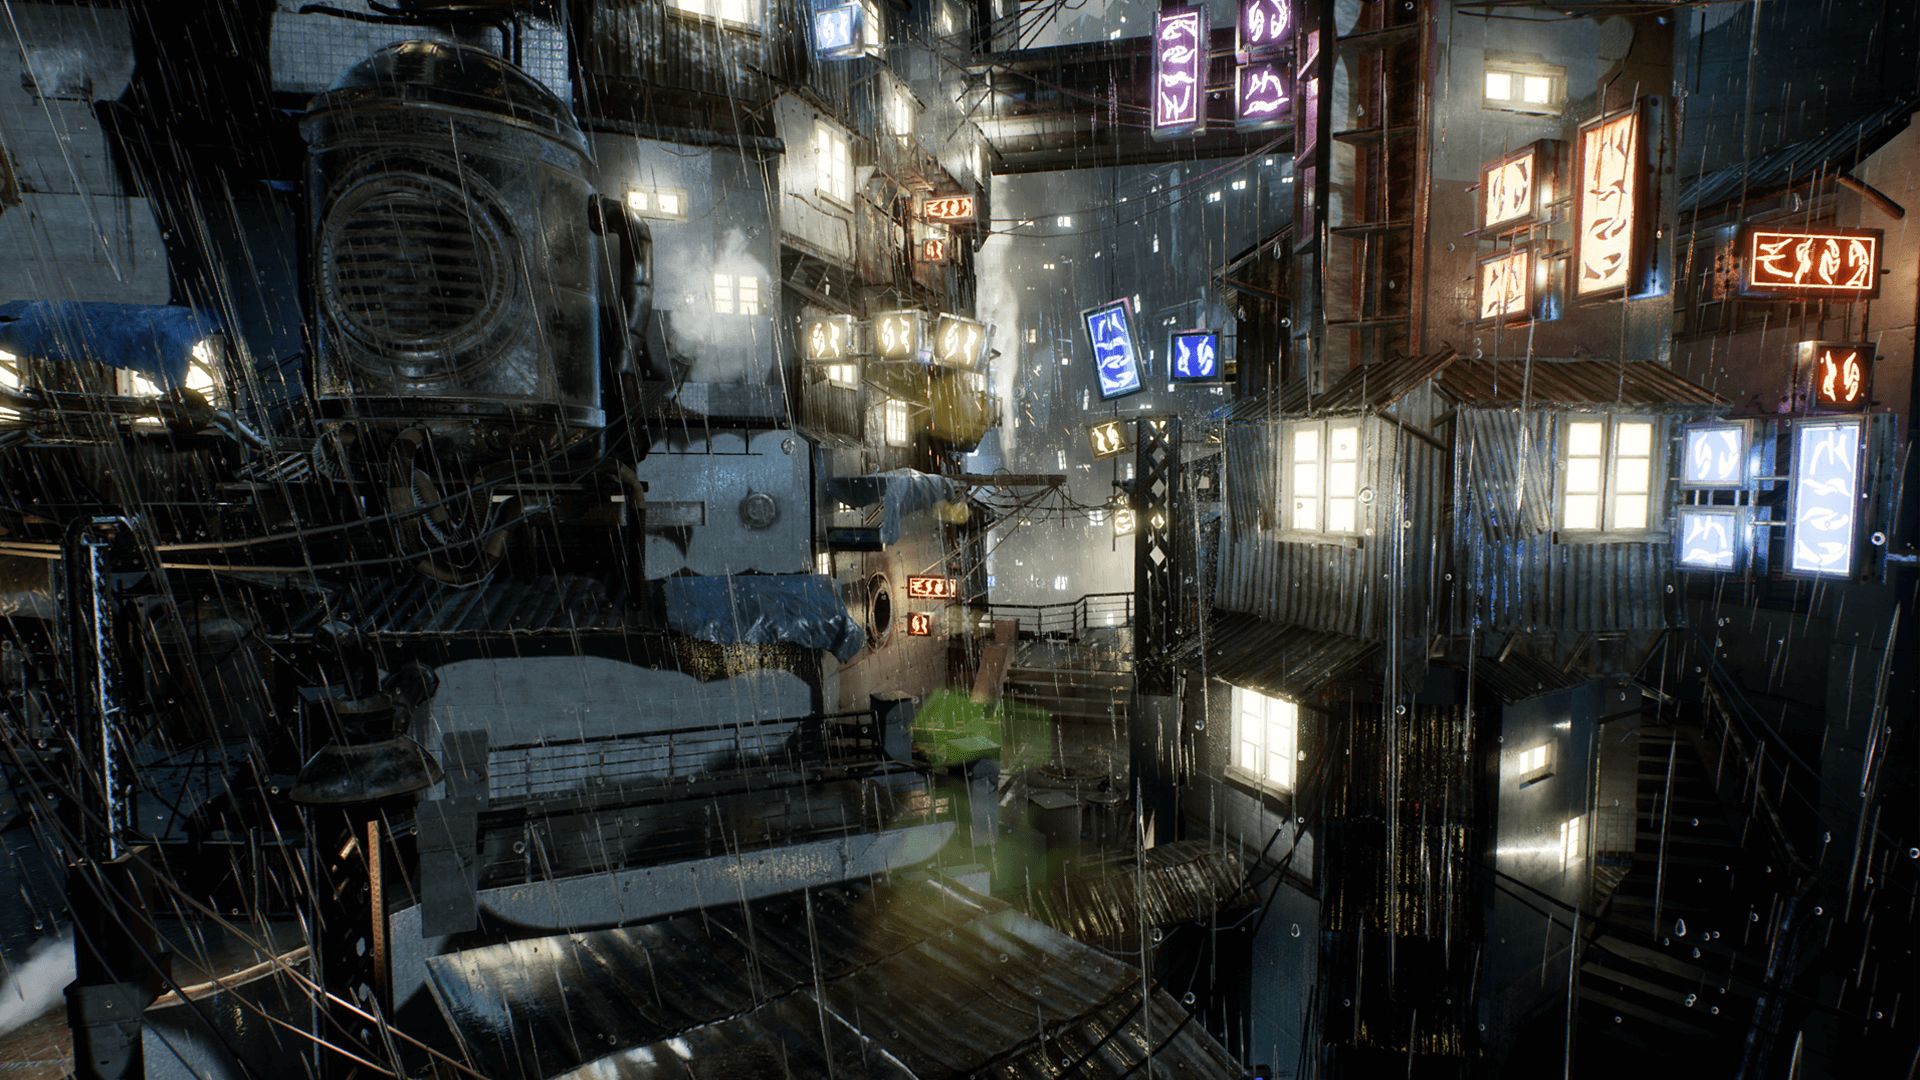
\includegraphics[scale=0.1]{images/city.png}

	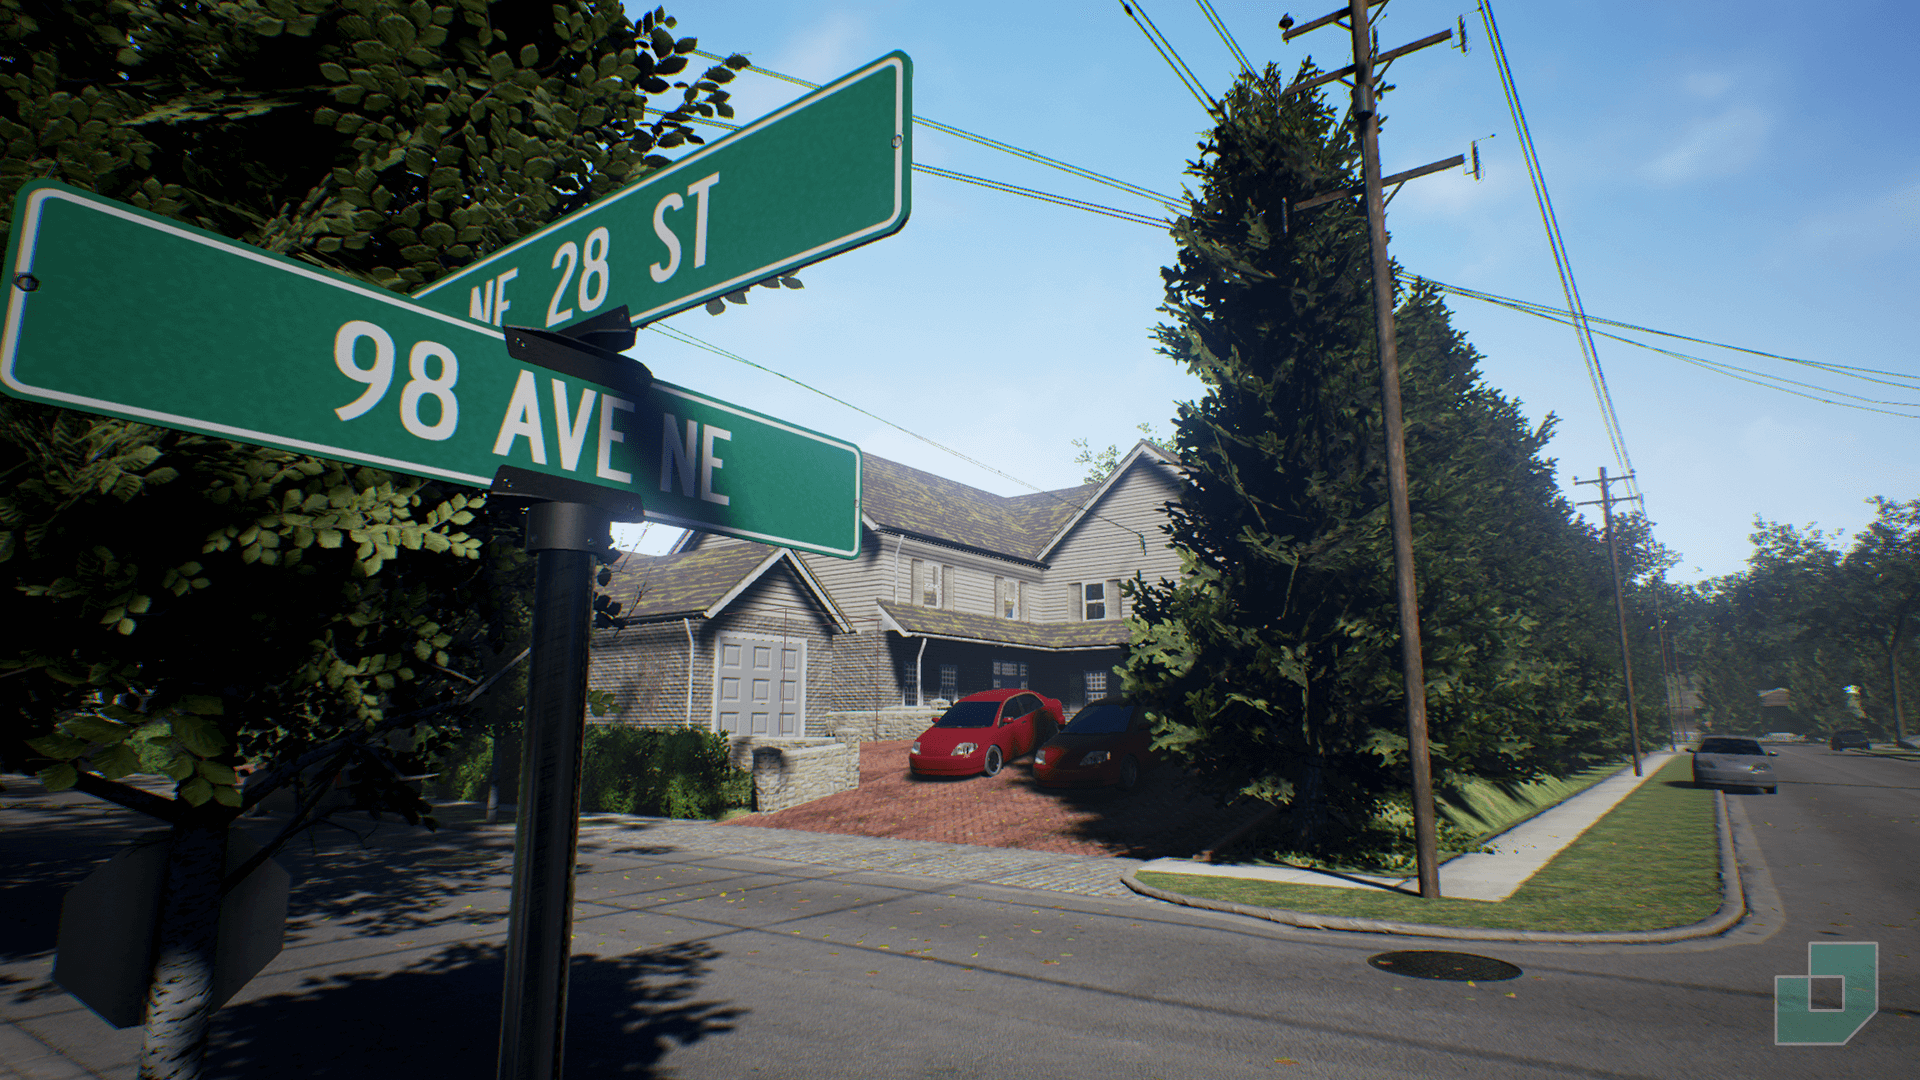
\includegraphics[scale=0.1]{images/neighborhood.png}
\end{frame}

\section{Applied tweaks}

\begin{frame}
	\frametitle{\insertsection}
	\begin{itemize}
	    \item {\bf Experience Replay.} History was collected, and experience was randomly sampled. That helped to reduce correlation in learning.
	    \item {\bf Freezed network to reduce correlation.} When computing updates, freezed version was used for estimation. This helps
	        to reduce bang of weights.
	    \item {\bf Huber Loss.} Huber loss is more robust
	        to outliars than MSE.
	    \item {\bf 4-frame delayed learning.}
	        Taking into account several frames helps network to understand
	        distance, velocity and acceleration better.
	\end{itemize}
\end{frame}

\section{Implemented Rewards}

\begin{frame}
	\frametitle{\insertsection}
	\begin{itemize}
    \item {\bf Exploration Reward.} Reward is described as $\frac{d - r}{\tau - r}$, where $d$ is distance, $r$ is radius, $\tau$ is constant.
        Also we penalize going too high.
    \item {\bf Path Reward.} We force collision avoidance to fixed lines, and penalize going far wary from them.
    \item {\bf Landscape Reward.} The aim is to reach the goal point in the environment. Therefore the reward is the difference $\text{dist}_{\text{prev}} - \text{dist}$ where $\text{dist}_{\text{prev}}$ is the distance to the goal in the previous state and $\text{dist}$ is distance to the goal in the current state.
    \item {\bf Corridor Reward.} We try to hardly penalize big changes in altitude(Z axis) as well as reward additional discovery via cityblock distance.
\end{itemize}
\end{frame}

\section{Implemented Action Spaces}

\begin{frame}
	\frametitle{\insertsection}
	\begin{itemize}
	    \item {\bf Grid Action Space.} Frontal camera image is separated into $M^2$ parts, which correspond to moving actions. Moving forward is
	        mandatory.
	    \item {\bf Canonical (Default) Action Space.} Forward, Backward, Up, Down, Left, Right, Stay.
	    \item {\bf Flat Action Space.} No up or down, rotations introduced.
	    \item {\bf Corridor Action Space.} This action space is just a default with added turns to give quadrotor ability to maneuver through the rather tight corners of the corridor.
	\end{itemize}
\end{frame}

\section{Exploration}

\begin{frame}
	\frametitle{\insertsection}
		\begin{itemize}
		    \item {\bf Constant $\varepsilon$-greedy.} Exploration is constant over time, or disabled (for evaluation).
		    \item {\bf Simulated annealing $\varepsilon$-greedy.} Exploration is scheduled by simulated annealing, and essentially decreases with time. Schedule is exponential.
		\end{itemize}
\end{frame}

\section{Results}

\begin{frame}
	\frametitle{\insertsection}
	Corridor:

	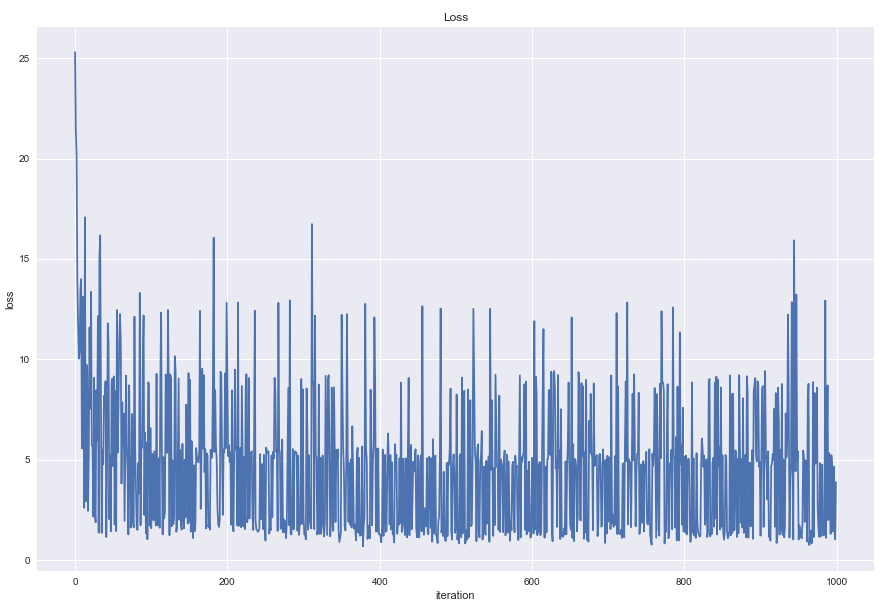
\includegraphics[height=0.43\textheight]{images/corridor_loss.png}
	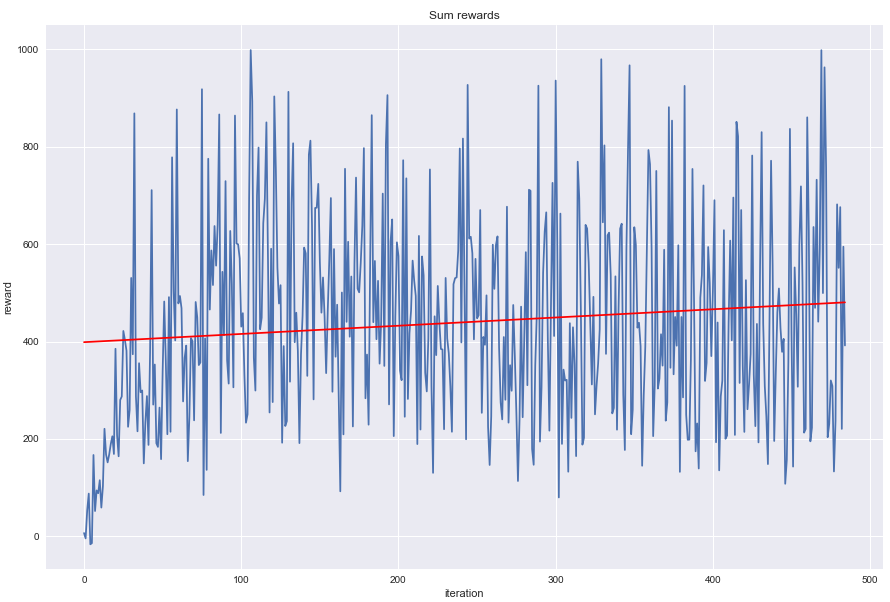
\includegraphics[height=0.43\textheight]{images/corridor_rewards.png}
\end{frame}

\begin{frame}
	\frametitle{\insertsection}
	Landscape:

	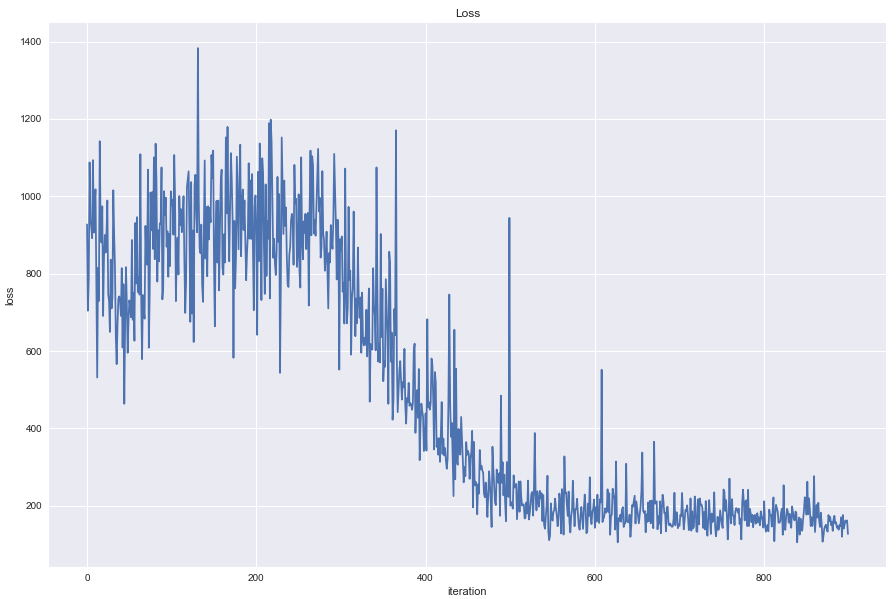
\includegraphics[height=0.43\textheight]{images/landscape_loss.png}
	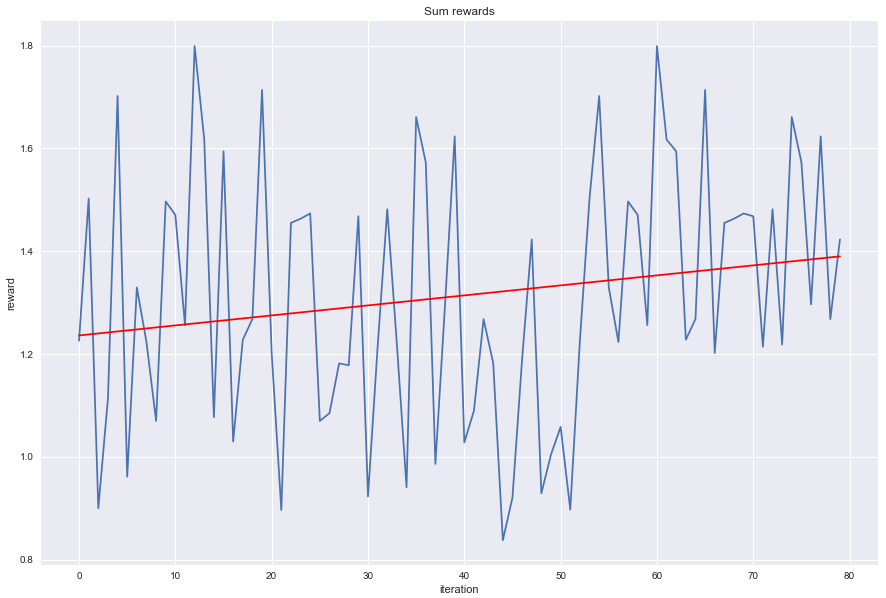
\includegraphics[height=0.43\textheight]{images/landscape_rewards.png}
\end{frame}

\section{Team Contribution}
\begin{frame}
	\frametitle{\insertsection}
	\begin{itemize}
    \item {\bf Aibek Alanov.} Architecture of the framework, Deep Agent reproduction,
        Adopting Unreal Engine to Linux, Landscape Mountains environemt,
        Landscape Reward, Flat Action Space, Constant and Annealing exploration,
        Report, Presentation.

    \item {\bf Aliaksandr Nekrashevich.} Project proposal, Achitecture of
        the framework, Deep Agent reproduction, Blocks Environment,
        Corridor Environment, Exploration and Path Rewards,
        Grid and Default Action Spaces, Report, Team Management.

    \item {\bf Dmitriy Salnikov.} Deep Agent reproduction, AirSim Tweaks,
        Unreal Engine on Windows, Environment convertation to Linux,
        Environment hand-crafting, Corridor Reward, Cave and Corridor
        Environments, Windows Environments, Exploration Strategies,
        Presentation.
\end{itemize}
\end{frame}

\begin{frame}
	\begin{center}
		{\huge\alert{Any questions?}}
	\end{center}
\end{frame}

\end{document}
